% !TEX root = ../YourName-Dissertation.tex

\chapter{Fast and Precise Side-channel Vulnerability Detection}\label{chapter3}
\section{Problem}
Side-channel attacks infer sensitive information such as cryptographic keys, personal data from software products unconsciously. Based on the discussions in \S\ref{chapter1} and \S\ref{chapter2}, patching leakage sites in software is usually easier than adopting new hardware to defend against side-channel attacks. In order to eliminate those leakage sites, developers also need to identify potential leakage sites from the code base manually. However, the manual process is tedious and error-prone. Recent studies~\cite{203878} also suggest fixing old vulnerabilities can sometimes introduce new leakages. 

Recent work has made good progress in identifying side-channel leakages automatically. Some tools (e.g., CacheD, CaSym) can successfully identify unknown leakage sites from software products automatically. However, those tools have the following limitations. 

First, although some tools can find side-channel leakages in real-world software products, they can only analyze one code fragment at a time due to the expensive performance overhead. As a result, users sometimes need to manually cut off some irrelevant code based on the user's experience. The trimming process is tedious and needs domain knowledge from users (e.g., which part of the code is more likely to have side-channel leakage sites). More importantly, those tools miss leakages on the trimmed code.

Second, many tools perform the analysis at the level of intermediate representations (IR) instead of machine code to facilitate the implementations. However, side-channel leakages are a pretty low-level issue and a low-level analysis can give the most accurate results. For example, the IR-level branches is not necessarily a superset or a subset of machine-code level branches. Besides, compiler optimizations can eliminate the IR-level branches like conditional moves and the converse could also happen. 

To overcome the problem, we propose a fast and precise method to detect the side-channel leakages in real-world software products. Different from previous methods, our tool analyzes on the machine code, which can give more precision than traditional IR-based approaches.  We examine the bottleneck of current symbolic execution approaches and optimize it to work on real-world cryptography systems. The evaluation results show that our tool can identify previous side-channel leakages, as well as find new leakages. Compared to recent tools, our tool is 3-100x faster while finding all the leakages when we evaluate on the same benchmarks.

\section{Background and Threat Model}
\subsection{Micro-architectures}
Many side-channel attacks are architecture-dependent. To facilitate the illustration, we present some necessary backgrounds in this section.

CPUs can process data much faster than the main memory (DRAM) can supply it. To bridge the performance gap between the CPUs and the main memory, modern CPUs adopt a hierarchy memory. By storing extra copies of data and code in a smaller but faster memory, the software can get its most recently accessed code and data in a shorter time.

Figure~\ref{fig:memory_hierarchy} shows the overview of the hierarchy memory. For a CPU with multiple Cores, each core has two private level-1 (L1) cache, an instruction cache (iCache) and a data cache (dCache). Because instructions and data have different access patterns, separating iCache and dCache make it possible CPUs to fetch the code and data simultaneously and improve the performance. Followed by the level-1 cache, each core also has the unified private level-2 cache. The level-3 cache is the last level cache (LLC). The LLC is shared among all the cores. The main memory is the bottom-most under the memory hierarchy. 
\begin{figure}
    \centering
    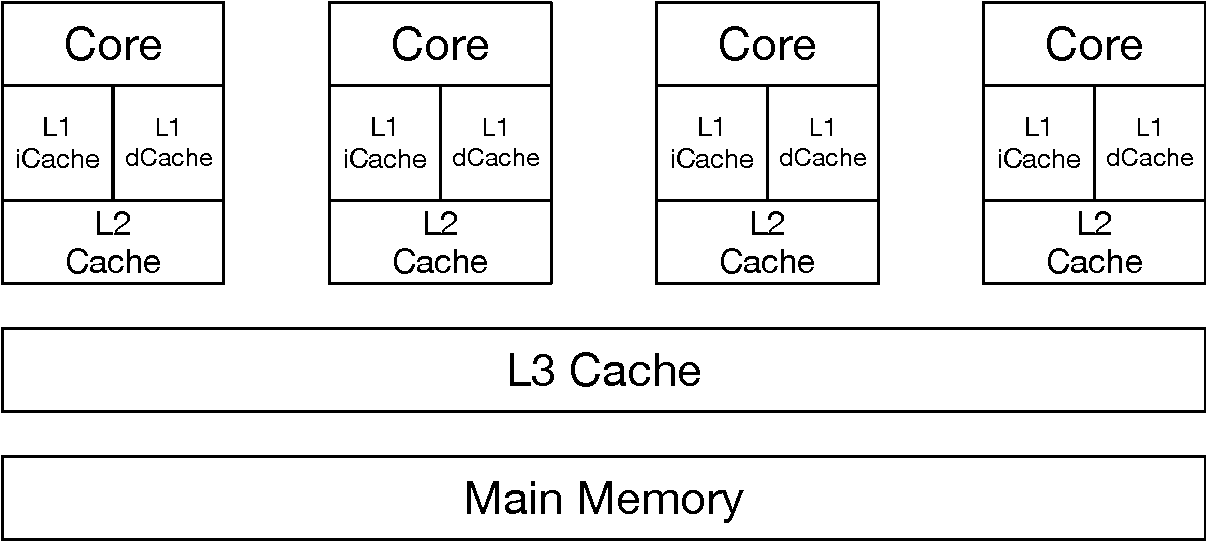
\includegraphics[width=.65\columnwidth]{./figures/chapter3/architecture.pdf}
    \caption{Computer Memory Hierarchy}\label{fig:memory_hierarchy}
\end{figure}

The current computer memory hierarchy opens the way for side-channel attacks from two aspects. First, the architecture relies on the system software to manage the addressing, which becomes a problem in a threat model where the operating system is not untrusted (e.g., Intel SGX). Second, the size of the cache is smaller than the main memory, which makes it possible that several program shares the same cache unit (e.g., cache line, cache set).

\begin{figure}
    \centering
    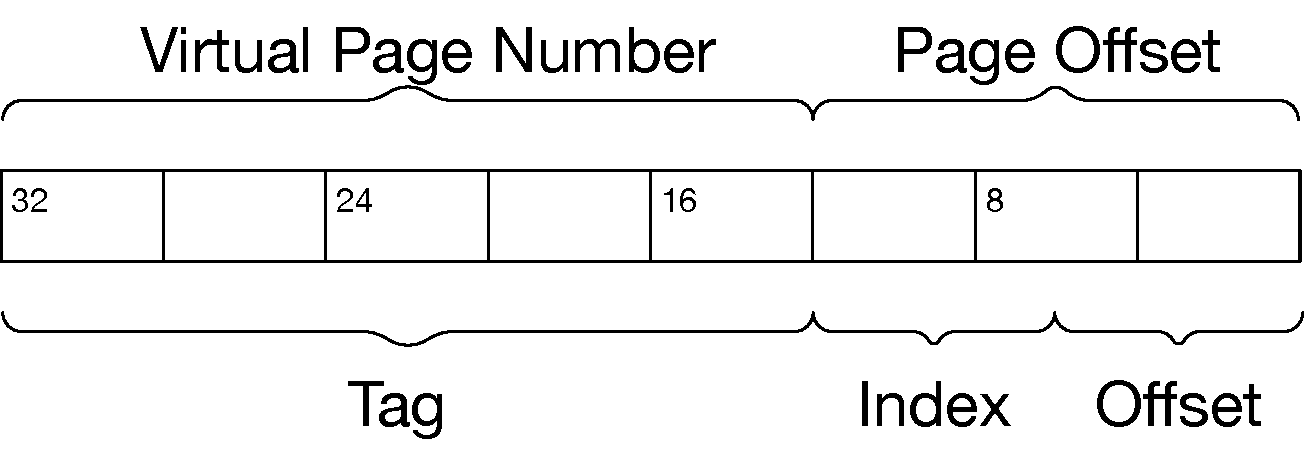
\includegraphics[width=.65\columnwidth]{./figures/chapter3/address.pdf}
    \caption{Memory Addressing}\label{fig:memory_address}
\end{figure}

In modern CPUs, L1 and L2 caches are traditional N-way set associate caches. That is, the cache is divided into several cache sets, and each set is associated with several cache lines. The cache line is the atomic unit. As shown in Figure~\ref{fig:memory_address}, when the cache is accessed, the CPU uses the \textsf{Index} field of the address to locate a cache set. After that, it tries to use the \textsf{Tag} field to match every cache line inside the set line. If the CPU can locate a cache line with the same tag, then a cache hit occurs. The CPUs use a similar process to manage the main memory. The main memory is divided into many pages. As shown in Figure~\ref{fig:memory_address}, 
the translation process keeps the bottom bits while use the top bits to map the Physical Page Numbers to Virtual Page Numbers.

\subsection{Threat Model}
We assume that an attacker shares the same hardware platform with the target.
The attacker attempts to retrieve sensitive information through address-based
side-channel attacks. The attacker has no direct access to the target's memory or cache,
but it can probe its memory or cache at each program point. 
Here are a few examples. 1) A host machine has several Virtual Machines (VMs). The victim runs the application inside one VM. An attacker can start a new VM and probe the process running on the other VM.  2) In a shielding system, a malicious operating system can extract sensitive information from the protected application. 3) An user level application can probe some sensitive information inside the kernel.

In reality, the
attacker will face many possible obstacles such as the noisy observations 
of the memory or cache. However, for this project, we assume
the attacker has noise-free observations as in previous work~\cite{203878,182946,Brotzman19Casym}. 
The threat model captures most cache-based and address-based side-channel attacks. 
We only consider deterministic programs and assume an attacker 
has access to the source code or binary executable of the target program.


\section{Illustrative examples}

\section{Our Theoretical Frameworks}
We now discuss how to model observations ($O$), which are the direct information
that an adversary can get during the attack.

During the execution, a program ($\beta$) have many temporary values ($t_i \in
T$). Once $\beta$ (program), $k$ (secret), and $m$ (message, public) are
determined, $t_i$ is also fixed. Therefore, $ t_i = f_i(\beta, k, m)$, where $f_
i$ is a function that maps between $t_i$ and ($\beta$, $k$, $m$).

In the paper, we consider two code patterns that can be exploited by an attacker,
\emph{secret-dependent control transfers} and \emph{secret-dependent data
accesses}. In other words, an adversary has observations based on control-flows
and data accesses.

\subsection{Secret-dependent Control Transfers}
We think a control-flow is secret-dependent if different input sensitive keys
($K$) can lead to different branch conditions. Therefore,
We define a branch is secret-dependent if:
$$\exists k_{i1}, k_{i2} \in K, \,f_i(\beta, k_{i1}, m) \neq f_i(\beta, k_{i2}, m)$$

An adversary can observe which branch the code executes, if the branch condition
equals to $t_b$. We use the constraint $c_i : f_i(\beta, k, m) = t_b$ to model
the observation ($o$) on secret-dependent control-transfers.

\subsection{Secret-dependent Data Accesses}
Similar to secret-dependent control-flow transfers, a data access operation is
secret-dependent if different input sensitive keys ($K$) can lead to different
memory addresses. We use the model from CacheD~\cite{203878}. The low $L$ bits
of the address are irrelevant in side-channels.

We consider a data access is secret-dependent if:
$$\exists k_{i1}, k_{i2} \in K, \,f_i(\beta, k_{i1}, m) >> L \neq f_i(\beta, k_{i2}, m) >> L$$

If the memory access equals to $t_b$, we can use the constraint $c_i :
f_i(\beta, k, m) >> L = t_b >> L$ to model the observation on secret-dependent
data accesses.

With the above definitions, we can model an attacker's observation by a series of math
formulas. For example, in Figure~\ref{fig:side-channel}, if an attacker observes
the code executes the branch 1, we have $c_5: k_1 + k_2 < 4$ to describe an
attacker's knowledge and $K^{o5} = \{k_1,\, k_2\,|\, (k_1 + k_2) < 4\}$. If an
attacker observes the code executes the branch 2, we have $c_8: k_1 - k_2 > 0$
and $K^{o8} = \{k_1,\, k_2\,|\, (k_1 - k_2) > 0\}$.
\section{Scalability}
\subsection{Trace-oriented Symbolic Execution}
While symbolic execution can capture fine-grained semantics of programs, it
is also notorious for its unbearable performance cost. Previous trace-oriented
symbolic execution based
works~\cite{203878,Chattopadhyay:2017:QIL:3127041.3127044} all have large
performance bottlenecks. As a result, those approaches either only apply to
small-size programs~\cite{Chattopadhyay:2017:QIL:3127041.3127044} or apply some
domain knowledge to simplify the analysis. 
%Those tools interpret each
%instruction and update memory cells and registers with formulas that
%captured the semantics of the execution and search different input values that
%can lead to different execution behaviors using constraint solver. 
We implement the approach presented in \S\ref{sec:trace-qif} and model the side-channels as formulas. While the tool can finish analyzing some simple cases like AES, it can
not handle complicated cases like RSA.
We observe that finding side-channels using symbolic execution is different from
traditional general symbolic execution and can be optimized to be as efficient
as other methods with approaches below.

\subsection{Interpret Instructions Symbolically}
Existing binary analysis tools~\cite{shoshitaishvili2016state,
10.1007/978-3-642-22110-1_37} usually translate machine instructions into
intermediate languages (IR) to simplify analysis. 
The reason is that the number of machine instructions is
enormous, and the semantics of each instruction is complex. Intel Developer
Manual~\cite{intelsys} introduces more than 1000 different x86 instructions. 
IR typically has fewer instructions compared to the original machine ISA\@.
However, the IR layer, which predigest the implementation
and reduce the workload of those tools, is not suitable for side-channels 
analysis. Memory-based side-channels are very low issues. So, in general,
IR-based or source code side-channels analyses are not accurate enough.
In many cases, compilers can use conditional moves or bitwise operations to eliminate
branches. Also, as some IRs are not a superset or a subset of ISA, 
it is hard to rule out conditional jumps introduced by IR and add real branches 
eliminated by IR transformations.

Moreover, the IR design introduces significant overhead~\cite{217563}.
Transferring machine instructions into IR is time-consuming. For example,
REIL IR~\cite{dullien2009reil}, adopted in CacheS~\cite{236338}, has multiple
transform processes, from binary to VEX IR, BAP IR, and finally REIL IR\@. 
Also, IR increases the total number of instructions. For example, x86
instruction \textit{test eax, eax} transfers into 18 REIL IR instructions. If we
assume the time of symbolically executing grows as the number of instructions increase, the
design of adopting IR layers can introduce large overhead.

\vspace*{2pt}
\textbf{Our Solution to Challenge C2:}
We adopt the approach from QSYM~\cite{217563} and implement the symbolic execution
directly on the top of x86 instructions. Table~\ref{scala:ir} shows that
eliminating the IR layer can reduce the number of instructions executed during
the analysis.

\begin{table}%[ht]
      \centering\small\footnotesize
      \caption{The number of x86,  % instructions and the number of 
             REIL IR, and VEX IR instructions on the traces of crypto programs.}
      \label{scala:ir}
      \resizebox{.7\columnwidth}{!}{%

            \begin{tabular}{cccc}
                  \hline
                                    & \begin{tabular}[c]{@{}c@{}}Number of\\ x86 Instructions\end{tabular} & \begin{tabular}[c]{@{}c@{}}Number of\\ VEX IR\end{tabular} & \begin{tabular}[c]{@{}c@{}}Number of\\ REIL IR\end{tabular} \\ \hline
                  AES OpenSSL 0.9.7 & $1,704$                   & $23,938$ (15x)            & $62,045$ (36x)            \\
                  DES OpenSSL 0.9.7 & $2,976$                   & $41,897$ (15x)            & $100,365$ (33x)           \\
                  RSA OpenSSL 0.9.7 & $1.6*10^7$                & $2.4*10^8$ (15x)          & $5.9*10^8$ (37x)          \\
                  RSA mbedTLS 2.5  & $2.2*10^7$                & $3.1*10^8$ (15x)          & $8.6*10^8$  (39x)         \\ \hline
            \end{tabular}
      }
\end{table}

\subsection{Constraint Solving}
As discussed in \S\ref{side-channel:condition}, the problem of identifying
side-channels can be reduced to the question below.

\begin{quote}
      \textit{Can we find two different input variables $k_1, k_2 \in K$ that
            satisfy the formula $f_a(k_1) \neq f_a(k_2)$?}
\end{quote}

Existing approach relies on satisfiability modulo theories (SMT) solvers (e.g,
Z3~\cite{DeMoura:2008:ZES:1792734.1792766}) to find satisfying $k_1$ and $k_2$.
We argue that while it is a universal approach to solving constraints with SMT
solvers, for constraints with the above formats, using custom heuristics and
testing is much more efficient in practice. Constraint solving is a decision
problem expressed in logic formulas. SMT solvers transfer the inputted SMT
formula into the boolean conjunctive normal form (CNF) and feed it into the
internal boolean satisfiability problem (SAT) solver. The translation process,
called ``bit blasting'', is time-consuming. Also, as the SAT problem is a
well-known NP-complete problem, it is also hard to deal when it comes to
realistic uses with huge formulas. Despite the rapid development of SMT solvers
in recent years, constraint solving remains one of the obstacles to achieve the
scalability for real-world crypto systems.

\vspace*{2pt}
\textbf{Our Solution to Challenge C3:}
Instead of feeding the formula $f_a(k_1) \neq f_a(k_2)$ into a SMT solver, we
just randomly pick up $k_1, k_2 \in K$ and test them if they can satisfy the
formula. Our solution is based on the following intuition. For most combination
of $(k_{1}, k_{2} )$, the formula $f_a(k_1) \neq f_a(k_2)$ holds. As long as
$f_a$ is not a constant function, such $k_1, k_2$ must exist. For example,
suppose each time we only have 5\% chance to find such $k_1, k_2$, then after we
test with different input combination with 100 times, we have $1 -
(1-0.05)^{100} = 99.6\%$ chance find such $k_1, k_2$. Such random algorithms
work well for our problem.

\section{Design and Implementation}
\subsection{Trace Logging}
The trace information can be logged via some emulators (e.g., QEMU) or dynamic binary instrumentation tools (DBI). 
We run a program with the concrete input under the DBI to record execution traces.
The trace data has the following information:
\begin{itemize}
     \item Each instruction mnemonics and its memory address.
     \item The operands of each instruction and their concrete values during the runtime.
     \item The value of EFLAGS register. 
     \item The memory address and the length of the sensitive information.
      Most crypto libraries stores sensitive information in arrays,
      variables or contiguous buffer.
\end{itemize}

\subsection{Instruction Level Symbolic Execution}
\label{InstructionSE}
The primary purpose of the step is to generate constraints of the input sensitive information from the execution trace. If we give the target program a new input which is different from the original input that was used to generate the execution trace but still satisfies those constraints, as an attacker, he will have the same observations on control-flow transfers and data-access patterns.

The tool runs symbolic execution on top of execution traces. At the beginning of the symbolic execution, the tool creates new symbols for each byte in the raw buffer. For other data in the register or memory at the beginning, we use actual values from the runtime information collected during the runtime. During the symbolic execution for each instruction, the tool updates every variable in the memory and registers with a math formula. The formula is made up of concrete values and the input key as the symbols accumulated through the symbolic execution.
For each formula, the tool will check weather it can be reduced into a concrete values (e.g., $k_1+12-k_1 = 12$ ). If so, the tool will only use the concrete values in the following symbolic execution.

\subsubsection{Verification and Optimization}
We run the symbolic execution (SE) on top of x86 instructions. In other words, we do not rely on any intermediate languages to simplify the implementation of symbolic execution. While the implementation itself has a lot of benefits (Better performance, accurate memory model), we need to implement the symbolic execution rules for each x86 instruction. 
However, due to the complexity of x86, it is inevitable to make mistakes. Therefore, we verify the correctness of the SE engine during the execution. 
The tool will collect the runtime information (Register values, memory values) and compare them with the formula generated from the symbolic execution. Whenever the tool finishes the symbolic execution of each instruction, the tool will compare the formula for each symbol and its actual value. If the two values do not match, we check the code and fix the error. Also, if the formula does not contain any symbols, the tool will use the concrete value instead of symbolic execution.

\subsubsection{Secret-dependent control-flows}
An adversary can infer sensitive information from secret dependent control-flows. There are two kinds of control-transfer instructions: the unconditional control-transfer instructions and the conditional transfer instructions.
The unconditional instructions, like CALL, JUMP, RET transfer control from one code segment location to another. Since the transfer is independent of the input sensitive information, an attacker was not able to infer any sensitive information from the control-flow. 
So the unconditional control-transfer does not leak any information based on our threat model. During the symbolic execution, we update the register information and memory cells with new formulas accordingly.

The conditional control-flow transfer instructions, like conditional jumps, depending on CPU states, may or may not transfer control flows. For conditional jumps, the CPU will test if certain condition flag 
(e.g., CF = 0, ZF =1) is met and jump to certain branches, respectively.
The symbolic engine will compute the flag and represent the flag in a symbol 
formula. Because we are running on a symbolic execution on an execution trace, we know which branch is executed.
If a conditional jump uses the CPU status flag, we will generate the constraint accordingly.

For examples, considering the below x86 code snippet,

\begin{lstlisting}
 ...
0x0000e781      add dword [local_14h], 1
0x0000e785      cmp dword [local_14h], 4
0x0000e789      jne 0xe7df
0x0000e78b      mov dword [local_14h], 0
 ...
\end{lstlisting}

At the beginning of the instruction segment, the value at the address of local\_14h can be written as $F(\vec{K})$. At the address $e785$, the value will be updated with $F(\vec{K})+1$. Then the code compares 
the value with 4 and use the result as a conditional jump. Based on the result, we can have the following formula:

$$F(\vec{K}) + 1 = 4$$

The formula, together with the memory address ($0xe789$) is store as a \textit{formula tuple (address, formula)}. Each formula tuple represents one leakage site.

\subsubsection{Secret-dependent data access}
Like input-dependent control-flow transfers, an adversary can also infer sensitive information from the data access pattern as well. We try to find this kind of leakages by checking every memory operand of the instruction. We generate the memory addressing 
formulas. As discussed before, every symbols in the formula is the input key. If the formula does not contain any symbols, the memory access is independent 
from the input sensitive information and will not leak any sensitive information according to our threat model. Otherwise, we will generate the constraint for
the memory addressing. We model the memory address with a symbolic formula $F(\vec{K})$. Because we also have the concrete value of the memory address $Addr1$. 
Inspired by the work from~\cite{203878}, the formula can be written as:

$$F(\vec{K}) >> L = Addr1 >> L$$

$L$ represents the minimum memory address granularity that an attacker can observe. For example, Flush and Reload can distinguish between different cache lines, which means the value of L is 6.

\subsubsection{Information Flow Check}
\tool{} is designed to help software developers find and understand the side-channel vulnerabilities. To ease the procedure of fixing the bug, we also track the information flow for each byte of the input
buffer. 
The step can be seen as the multiple-tag taint analysis. With the help of the information from symbolic execution, we can implement a relatively simple but relatively precise information flow track.
At the beginning of the analysis, \tool{} keep a track for each byte in 
the original buffer. When \tool{} symbolically executes each instruction in the trace, it will check every value read from registers or memory. If the value is concrete, it means the instruction has nothing to do with the original buffer.
If the value is a formula, it means the original information passes through the instruction. Since each byte in the sensitive buffer is represented as a symbol with a unique ID, \tool{} can know which byte in the origin buffer goes through the instruction.

\section{Evaluation}

\section{Discussion}

